\documentclass[11pt,a4paper]{article}

% ============================================================
%  Perfiles bancarios en Argentina — Trabajo Final
%  Taller de Tesis I — Entrega IV
%  Victoria Di Liscia — Maestría en Explotación de Datos, FCEN-UBA
% ============================================================

\usepackage[utf8]{inputenc}
\usepackage[T1]{fontenc}
\usepackage[spanish,es-noquoting]{babel}
\usepackage{lmodern}
\usepackage[a4paper,margin=2.5cm]{geometry}
\usepackage{graphicx}
\usepackage{booktabs}
\usepackage{amsmath,amssymb}
\usepackage{xcolor}
\usepackage{caption}
\usepackage{enumitem}
\usepackage{fancyhdr}
\usepackage{titlesec}
\usepackage{natbib}
\usepackage[hidelinks,colorlinks=true,linkcolor=azultesis,citecolor=azultesis,urlcolor=rojotesis]{hyperref}

% ---- Paleta (colorblind-friendly, función comunicativa) ----
\definecolor{azultesis}{RGB}{31,73,125}
\definecolor{rojotesis}{RGB}{170,50,60}
\definecolor{gristesis}{RGB}{90,90,90}

% ---- Encabezado / pie ----
\pagestyle{fancy}
\fancyhf{}
\fancyhead[L]{\small\textcolor{gristesis}{Perfiles bancarios en Argentina}}
\fancyhead[R]{\small\textcolor{gristesis}{Trabajo Final}}
\fancyfoot[C]{\thepage}
\renewcommand{\headrulewidth}{0.4pt}

% ---- Estilo de secciones ----
\titleformat{\section}{\color{azultesis}\Large\bfseries}{\thesection}{0.6em}{}
\titleformat{\subsection}{\color{azultesis}\large\bfseries}{\thesubsection}{0.6em}{}
\titleformat{\subsubsection}{\color{azultesis}\normalsize\bfseries}{\thesubsubsection}{0.6em}{}

\captionsetup{labelfont={color=rojotesis,bf},font=small}
\setlist{itemsep=2pt,topsep=3pt}

% ---- Caja de nota ----
\usepackage{tcolorbox}
\newtcolorbox{notebox}{colback=azultesis!4,colframe=azultesis!40,boxrule=0.5pt,arc=2pt,left=6pt,right=6pt,top=4pt,bottom=4pt}

% ============================================================
\begin{document}

% ------------------- PORTADA -------------------
\begin{titlepage}
\centering
\vspace*{3cm}
{\color{azultesis}\rule{\textwidth}{1.2pt}}\\[0.4cm]
{\Huge\bfseries\color{azultesis} Perfiles bancarios en Argentina}\\[0.3cm]
{\Large\color{rojotesis} Una segmentación no supervisada del sistema financiero}\\[0.3cm]
{\color{azultesis}\rule{\textwidth}{1.2pt}}\\[1.5cm]

{\large\bfseries Victoria Di Liscia}\\[0.6cm]
{Maestría en Explotación de Datos y Descubrimiento del Conocimiento}\\
{Facultad de Ciencias Exactas y Naturales --- Universidad de Buenos Aires}\\[1.5cm]

\begin{tabular}{rl}
\textbf{Asignatura} & Taller de Tesis I\\
\textbf{Instancia} & Trabajo Final (Entrega IV)\\
\textbf{Fecha} & Julio 2026\\
\end{tabular}

\vfill
\begin{notebox}
\small
\textbf{Nota sobre el código.} El código fuente completo (script de \textit{scraping} y
notebooks del análisis, con instrucciones de reproducibilidad y versiones de software)
se encuentra en el repositorio público del proyecto, referenciado en el Anexo (Sección~\ref{sec:anexos}).
Este documento no incluye código: las salidas relevantes se presentan como tablas y figuras.
\end{notebox}
\end{titlepage}

\tableofcontents
\newpage

% ============================================================
\section{Introducción}
% ============================================================

\subsection{Contexto y motivación}

El sistema bancario argentino reúne alrededor de 70 entidades de naturaleza
heterogénea ---bancos públicos nacionales y provinciales, privados nacionales, filiales
de bancos extranjeros y entidades de nicho--- cuyas diferencias en modelos de negocio no
son capturadas por los promedios agregados del sistema que publica regularmente el BCRA.
Un banco público provincial con red de sucursales y fondeo de depósitos minoristas, un
banco de inversión que opera en el mercado de capitales y una \textit{fintech} 100\,\%
digital conviven bajo la misma categoría regulatoria de ``entidad financiera'', pero
responden a lógicas de negocio, estructuras de balance y exposiciones al riesgo distintas.
Identificar perfiles diferenciados en términos de balance, rentabilidad y riesgo crediticio
tiene implicancias directas para la política macroprudencial: permite diseñar
marcos regulatorios más precisos, anticipar cómo distintos tipos de entidades responden a
\textit{shocks} macroeconómicos y monitorear la aparición de modelos de negocio emergentes.

Si bien la literatura internacional sobre \textit{clustering} bancario es robusta
\citep{roengpitya2014,mercadier2025}, su aplicación al caso argentino permanece escasa.
La heterogeneidad del sistema local sugiere que los perfiles que emergerían de un análisis
de este tipo serían sustantivamente distintos a los documentados en economías desarrolladas,
lo que convierte a la Argentina en un caso de estudio de interés propio y no en una mera
replicación. Las técnicas modernas de aprendizaje automático permiten, además, ir más allá
de la identificación de grupos, explicando qué variables financieras los definen y con qué
peso relativo.

\subsection{Pregunta de investigación}

\begin{quote}
\textit{¿Existen perfiles diferenciados de bancos en Argentina según balance, rentabilidad
y riesgo? ¿Qué variables determinan cada perfil?}
\end{quote}

\noindent El trabajo aborda esta pregunta mediante segmentación no supervisada sobre datos
públicos del BCRA del período 2023--2025, integrando por primera vez para el caso argentino
información de balance con indicadores de oferta comercial pública, y validando la partición
resultante con un clasificador supervisado.

\subsection{Estructura del documento}

El documento sigue el flujo del \textit{pipeline} analítico. El marco teórico
(Sección~\ref{sec:marco}) releva antecedentes y técnicas. La declaración de objetivos e
hipótesis (Sección~\ref{sec:objetivos}) formaliza lo que el trabajo se propone. La
metodología (Sección~\ref{sec:metodologia}) describe datos, preprocesamiento, análisis
exploratorio y el diseño de modelado. Los resultados y la discusión
(Sección~\ref{sec:resultados}) presentan la segmentación, su validación supervisada y la
interpretación. La conclusión (Sección~\ref{sec:conclusion}) sintetiza hallazgos y trabajo
futuro. Los anexos (Sección~\ref{sec:anexos}) remiten al código y al material complementario.

% ============================================================
\section{Marco teórico}
\label{sec:marco}
% ============================================================

\subsection{Relevamiento de trabajos previos}

La literatura sobre segmentación bancaria no supervisada ofrece a este trabajo tres aportes
concretos, que se traducen en decisiones de diseño: cómo seleccionar las variables que entran
al algoritmo, cómo manejar la redundancia entre ratios, y cómo validar que la partición es
significativa. Se seleccionaron tres referencias que cubren, respectivamente, el diseño de
variables, la secuencia metodológica y el precedente más cercano en contexto.

\paragraph{Roengpitya, Tarashev \& Tsatsaronis (2014).}
En \textit{Bank business models} \citep{roengpitya2014} se identifican tres modelos de negocio
diferenciados ---banca minorista, banca mayorista de fondeo y banca de inversión orientada al
\textit{trading}--- sobre una muestra de 222 bancos internacionales, aplicando \textit{clustering}
jerárquico de Ward sobre ratios de balance. Su aporte central es la distinción metodológica entre
variables de elección (decisiones estratégicas del banco como estructura de
balance o mix de fondeo) y variables de resultado (rentabilidad, costos) que en el
esquema original se reservan para caracterizar los perfiles \textit{a posteriori}, evitando la
circularidad de definir grupos con las mismas dimensiones con que luego se los evalúa. Este trabajo
adapta dicho esquema: dado el tamaño reducido de la
muestra y la presencia de solapamientos entre perfiles, se incorpora un subconjunto acotado de
variables de resultado directamente al espacio de \textit{clustering}, controlando la posible
circularidad mediante la validación supervisada posterior.

\paragraph{Mercadier, Tarazi, Armand \& Lardy (2025).}
En \textit{Monitoring bank risk around the world using unsupervised learning}
\citep{mercadier2025} rankean 256 bancos de 43 países combinando 72 indicadores que reducen a 10
factores mediante PCA antes de aplicar \textit{k-means}. Aportan dos elementos: respaldo
para usar PCA como paso previo al \textit{clustering} cuando hay muchas variables
correlacionadas, y un marco de validación interna basado en \textit{silhouette} y
Davies-Bouldin como métricas complementarias. Este trabajo adopta ese marco con una salvedad: cuando existen bancos en zonas de frontera entre perfiles,
el \textit{silhouette} tiende a ser bajo aunque la partición sea válida, por lo que se complementa
con validación supervisada.

\paragraph{Chherawala, Vaidya \& Basu (2025).}
En \textit{Multidimensional surveillance of the Indian banking system} \citep{chherawala2025}
se aplica \textit{k-means} al sistema bancario indio (30 bancos, 2005--2023), comparando perfiles de
riesgo entre bancos públicos y privados a lo largo de episodios de estrés financiero. Es el
precedente más cercano en escala muestral y contexto institucional ---economía emergente, presencia
estatal significativa, dimensión muestral comparable a la argentina ($n \approx 30$--$50$)--- y
posiciona al \textit{clustering} como instrumento de supervisión macroprudencial, que es el horizonte
aplicado de esta tesis.

\paragraph{Diálogo entre los antecedentes y el caso argentino.}
Los tres trabajos comparten una convicción, que la heterogeneidad bancaria se organiza en un número reducido de modelos de negocio recuperables por métodos no supervisados, pero difieren en escala y en supuestos que el caso argentino tensiona. \citet{roengpitya2014} trabajan con grandes bancos internacionales, donde los tres modelos (minorista, mayorista de fondeo, inversión) emergen nítidos porque las entidades son grandes y especializadas; en un sistema chico y con fuerte presencia estatal como el argentino, esa nitidez se pierde y aparecen bancos ``híbridos'' en zonas de frontera. La estrategia de PCA + \textit{k-means} de \citet{mercadier2025} está pensada para muestras grandes ($n = 256$) donde el \textit{silhouette} es un criterio confiable; con $n = 52$ y perfiles solapados, esa métrica pierde poder de decisión, una limitación que este trabajo aborda de frente incorporando una etapa de validación supervisada. El precedente de \citet{chherawala2025} es el más transferible por contexto, pero se limita a variables de balance; ninguno de los tres antecedentes integra la oferta comercial de productos, que en el caso argentino resulta ser una dimensión discriminante, en particular para separar la banca minorista tradicional de la banca de inversión y para identificar el sub-grupo digital emergente. En síntesis, este trabajo hereda el marco metodológico de la literatura pero lo adapta a un sistema más chico, más heterogéneo y con una dimensión comercial que los antecedentes no contemplan.

\subsection{Conceptos y técnicas de ciencia de datos utilizados}

\begin{itemize}
  \item \textbf{Reducción dimensional --- PCA.} Transforma variables correlacionadas en componentes
  ortogonales que retienen la mayor parte de la varianza; mitiga la multicolinealidad antes del
  \textit{clustering} y revela la estructura latente del sistema.
  \item \textbf{Clustering.}
  \begin{itemize}
    \item \textit{K-Means:} partición que minimiza la suma de cuadrados intracluster; eficiente y
    equilibrada, requiere fijar $k$.
    \item \textit{GMM (Gaussian Mixture Model):} modelo probabilístico que asigna a cada banco una
    probabilidad de pertenencia a cada grupo, útil para caracterizar bancos en zonas de
    frontera. La implementación proviene de \texttt{scikit-learn} \citep{scikit-learn}.
    \item \textit{Ward (jerárquico) y DBSCAN (densidad):} usados como contraste para verificar que
    la partición no es un artefacto del algoritmo.
  \end{itemize}
  \item \textbf{Validación supervisada.}
  \begin{itemize}
    \item \textit{LightGBM} \citep{lightgbm}: \textit{gradient boosting} sobre árboles, entrenado
    sobre las etiquetas de \textit{cluster} para comprobar que los grupos son estadísticamente
    diferenciables.
    \item \textit{Validación cruzada anidada:} estimación honesta de generalización con muestras
    chicas, separando la selección de hiperparámetros de la evaluación.
  \end{itemize}
  \item \textbf{Interpretabilidad --- SHAP} \citep{lundberg2017}. Valores de Shapley que cuantifican
  la contribución de cada variable a la predicción, identificando qué ratios definen cada
  \textit{cluster}.
\end{itemize}

\subsection{Posicionamiento y aporte de la tesis}

Este trabajo retoma el esquema \textit{choice/outcome} de \citet{roengpitya2014} y la secuencia metodológica de \citet{mercadier2025}, que consiste en una etapa de reducción dimensional, seguida de una etapa de \textit{clustering} y, finalmente, una etapa de validación, y agrega tres elementos propios. En primer lugar, incorpora la oferta comercial pública relevada a partir del Régimen de Transparencia como una dimensión adicional de segmentación, que se suma a las variables de balance ya contempladas por los antecedentes. En segundo lugar, suma una etapa de validación supervisada con LightGBM, que permite confirmar de manera independiente que los grupos identificados por el \textit{clustering} son efectivamente diferenciables entre sí, y no producto del azar o de una partición arbitraria. En tercer lugar, utiliza SHAP para identificar qué variables resultan más relevantes a la hora de definir cada \textit{cluster}, lo que aporta una capa de interpretabilidad ausente en los antecedentes revisados. La combinación de estos dos últimos elementos, es decir, la validación supervisada y la interpretabilidad aplicada sobre las etiquetas surgidas del \textit{clustering}, constituye el principal aporte metodológico de este trabajo.

% ============================================================
\section{Objetivos e hipótesis}
\label{sec:objetivos}
% ============================================================

\subsection{Objetivos}

\paragraph{Objetivo general.} Identificar y caracterizar perfiles diferenciados de bancos en Argentina
mediante técnicas de segmentación no supervisada, integrando información de balance con indicadores de
oferta comercial pública para el período 2023--2025.

\paragraph{Objetivos específicos.}
\begin{itemize}
  \item Construir un \textit{dataset} integrado que combine indicadores de balance con información de
  oferta comercial pública del Régimen de Transparencia del BCRA.
  \item Describir la heterogeneidad estructural del sistema bancario argentino.
  \item Aplicar y comparar algoritmos de \textit{clustering} para detectar agrupamientos que no
  necesariamente coincidan con la clasificación administrativa por tipo de entidad.
  \item Caracterizar cada \textit{cluster} emergente por sus dimensiones económicas: rentabilidad,
  riesgo crediticio, estructura de fondeo, escala y oferta comercial.
  \item Validar la partición resultante con un clasificador supervisado e interpretar los perfiles con
  valores SHAP, identificando las variables que definen cada uno.
\end{itemize}

\subsection{Hipótesis de trabajo}

Al tratarse de un estudio de naturaleza exploratoria basado en aprendizaje no supervisado, el trabajo
se organiza en torno a una hipótesis general de trabajo, sujeta a verificación empírica:

\begin{notebox}
\textbf{Hipótesis general.} El sistema bancario argentino se organiza en un número reducido de perfiles
de negocio diferenciados y estables, que \textbf{no coinciden} con la clasificación administrativa por
tipo de entidad (público / privado nacional / extranjero), y que pueden caracterizarse de forma
interpretable a partir de un conjunto acotado de variables de balance y de oferta comercial.
\end{notebox}

\noindent Esta hipótesis es contrastable en dos sentidos, que se retoman a lo largo de las siguientes secciones. En primer lugar, si el tipo de entidad estructurara los grupos, los \textit{clusters} coincidirían con las categorías administrativas, algo que se verifica en la Sección~\ref{sec:res1} mediante la comparación directa entre las etiquetas obtenidas y la clasificación institucional de cada banco. En segundo lugar, si los perfiles fueran meros artefactos del algoritmo, un clasificador supervisado independiente no lograría reproducirlos con un desempeño superior al azar, lo que se evalúa en la Sección~\ref{sec:res2} a partir de los resultados de validación con LightGBM.

% ============================================================
\section{Metodología}
\label{sec:metodologia}
% ============================================================

\subsection{Presentación y descripción de los datos}
El \textit{dataset} integra dos fuentes públicas del BCRA que capturan dimensiones complementarias del
negocio bancario: el balance contable (qué tiene y cómo se fondea cada banco) y la oferta comercial
(qué productos ofrece y bajo qué condiciones). Esta combinación busca superar una limitación habitual
en la literatura de segmentación bancaria, que suele apoyarse exclusivamente en variables de balance
sin incorporar información sobre el comportamiento comercial efectivo de las entidades.
\begin{itemize}
  \item \textbf{Portal de entidades financieras:} estados contables, situación de deudores y datos de
  estructura (dotación de personal). Capturado mediante un \textit{scraper} propio para 56 bancos en
  tres cortes anuales (Dic-23, Dic-24, Dic-25).
  \item \textbf{Régimen de Transparencia} (Sección 36 de la normativa BCRA): siete archivos con
  información comercial estandarizada sobre hipotecas, préstamos personales, prendarios, plazo fijo,
  tarjetas, paquetes y cajas de ahorro. Cubre 51 de los 56 bancos (5 entidades no publican).
\end{itemize}
La unión por código BCRA y la consolidación de los archivos de transparencia producen un
panel transversal de 168 observaciones (56 bancos $\times$ 3 cortes) con 157 variables crudas.
Este volumen de variables refleja la heterogeneidad de formatos entre las siete fuentes de
transparencia, que fue necesario estandarizar antes de la consolidación. Sobre el balance se
construyeron 13 ratios estándar agrupados en seis dimensiones económicas (Cuadro~\ref{tab:ratios}).

\begin{table}[htbp]
\centering
\caption{Ratios financieros construidos, por dimensión económica.}
\label{tab:ratios}
\small
\begin{tabular}{ll}
\toprule
\textbf{Dimensión} & \textbf{Ratios} \\
\midrule
Rentabilidad & ROA, ROE \\
Apalancamiento & Activo / Patrimonio neto \\
Estructura de fondeo & Depósitos / Activo, Préstamos / Activo \\
Liquidez & (Efectivo + depósitos en bancos) / Depósitos \\
Eficiencia & Gastos de administración / Margen (\textit{cost-to-income}) \\
Riesgo crediticio & Cartera irregular (situaciones 3-4-5) \\
Productividad & Activo / Empleado \\
\bottomrule
\end{tabular}
\end{table}

\subsection{Preprocesamiento y limpieza}

El diagnóstico de calidad identifica las siguientes situaciones, ninguna atribuible a errores en el
proceso de recolección de datos:

\begin{itemize}
  \item Cinco bancos no publican el Régimen de Transparencia, por lo que la oferta comercial queda
  parcialmente faltante para $\sim$9\,\% de la muestra.
  \item Algunos bancos pequeños no reportan dotación de personal en todos los cortes, lo cual afecta
  el cálculo del ratio activo/empleado para esas entidades.
  \item Entidades de muy reciente operación (digitales) tienen series incompletas en Dic-23.
  \item A los 4 mayoristas sin cartera minorista relevante (Bank of China, JPMorgan, BNP Paribas,
  Cetelem) se les asigna \texttt{NaN} en lugar de 0 en cartera irregular, para que no aparezcan como
  ``0\,\% de mora'' y distorsionen las medianas por tipo.
  \item No se detectaron datos corruptos. Los valores extremos de ROA/ROE responden a fenómenos
  económicos reales: pérdidas de algunos extranjeros en 2024 y el fin del ciclo de LELIQ, documentado
  por el propio regulador \citep{bcra2024ief}. El rango de
  activo va de $\sim$7\,M a $\sim$48.000\,M de pesos (ratio 7.000$\times$), lo que obliga a trabajar en
  escala logarítmica y a usar la mediana en lugar de la media en las comparaciones por grupo.
\end{itemize}

Los valores faltantes en las variables de modelado se imputan por la mediana del panel, criterio robusto
a valores extremos.

\subsection{Análisis exploratorio de datos}

El análisis exploratorio cumple dos funciones: documentar la heterogeneidad del sistema y orientar el
modelado (qué transformar, qué excluir, qué variables aportan señal).

\paragraph{Estructura y concentración.} El sistema es estructuralmente competitivo pero con una leve tendencia a concentrarse: el índice de
Herfindahl-Hirschman (HHI) sobre activo pasa de 1.005 (Dic-23) a 1.056 (Dic-25) y la cuota de mercado
de los cinco mayores bancos sube de 59,1\,\% a 61,4\,\%. Ningún tramo del período supera el umbral de
concentración moderada (1.500), lo que indica que el sistema se mantiene dentro de un rango de baja
concentración a lo largo de todo el período analizado. El activo mediano por tipo de entidad (Dic-24)
es de 1.085\,M para los bancos públicos, 216\,M para los privados nacionales y 476\,M para los
extranjeros: el activo mediano de los bancos públicos resulta aproximadamente cinco veces mayor que
el de los privados nacionales, y poco más del doble que el de los extranjeros. Esta dispersión
de tamaño confirma la necesidad de tratar la escala como variable de control mediante el logaritmo
del activo.

\paragraph{Correlación entre ratios (Spearman, Dic-24).} La matriz de correlación
(Figura~\ref{fig:spearman}) revela tres bloques de alta colinealidad que justifican empíricamente reducir
la dimensión antes de clusterizar: \textit{escala} (activo, patrimonio y dotación con $\rho$ entre 0,91 y
0,97), \textit{rentabilidad} (ROA y ROE con $\rho = 0{,}92$) y \textit{fondeo} (apalancamiento y
depósitos/activo con $\rho = 0{,}65$). La eficiencia correlaciona negativamente con escala ($-0{,}61$) y
con rentabilidad ($-0{,}58$), confirmando su rol de ratio de costos: los bancos más grandes y rentables
son, en el sistema argentino, los más eficientes. Estos bloques anticipan una advertencia metodológica:
alimentar el \textit{clustering} con las 13 variables crudas equivaldría a ponderar tres veces la
dimensión ``escala'' y dos veces la ``rentabilidad'', sesgando la partición hacia esos ejes; de ahí la
transformación y el escalado robusto que se describen en la Sección~\ref{sec:tecnicas}.

\begin{figure}[htbp]
\centering
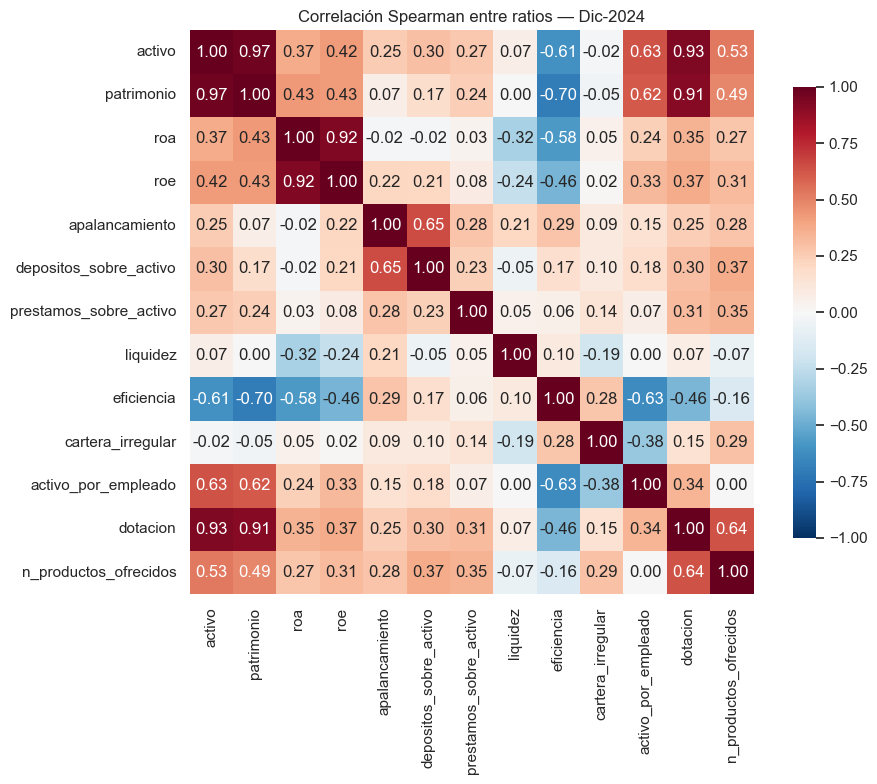
\includegraphics[width=0.72\textwidth]{figs_entrega3/fig_eda_spearman.png}
\caption{Matriz de correlación de Spearman entre los 13 ratios (Dic-24). Los colores intensos marcan los
tres bloques de alta colinealidad ---escala, rentabilidad y fondeo--- y la correlación negativa de la
eficiencia con escala y rentabilidad. La estructura de bloques justifica la reducción dimensional previa
al \textit{clustering}.}
\label{fig:spearman}
\end{figure}

\paragraph{Validación inferencial (Kruskal-Wallis, Dic-24).} Para verificar formalmente que los ratios separan a los tres tipos de entidad ($n = 17$ públicos,
30 privados nacionales y 9 extranjeros), se aplicó el test no paramétrico de Kruskal-Wallis. Seis de
ocho ratios rechazan la hipótesis nula al 5\,\% (Cuadro~\ref{tab:kw}). La liquidez es el ratio de
mayor poder discriminante, con una mediana de 33,1\,\% en los bancos extranjeros frente a 13,5\,\%
en los públicos. El hecho de que depósitos/activo y activo/empleado no separen univariadamente
anticipa un hallazgo clave del trabajo: el tipo administrativo no alcanza a captar por sí solo el
modelo de negocio de cada entidad, ya que dentro de un mismo tipo administrativo coexisten perfiles
comerciales y financieros distintos.

\begin{table}[htbp]
\centering
\caption{Test de Kruskal-Wallis por ratio (Dic-24). H$_0$: las tres distribuciones provienen de la misma
población.}
\label{tab:kw}
\small
\begin{tabular}{lrrc}
\toprule
\textbf{Variable} & \textbf{H} & \textbf{p-valor} & \textbf{Sig. 5\,\%} \\
\midrule
Liquidez              & 13,33 & 0,0013 & \checkmark \\
Apalancamiento        & 9,10  & 0,0106 & \checkmark \\
ROA                   & 6,85  & 0,0325 & \checkmark \\
Cartera irregular     & 6,67  & 0,0356 & \checkmark \\
N.º productos ofrecidos & 6,43 & 0,0401 & \checkmark \\
ROE                   & 6,20  & 0,0451 & \checkmark \\
Depósitos / Activo    & 3,95  & 0,1386 & --- \\
Activo / empleado     & 1,65  & 0,4391 & --- \\
\bottomrule
\end{tabular}
\end{table}

La lectura visual de las distribuciones por tipo de entidad (Figura~\ref{fig:boxplots}) refuerza este
punto. Aun en los ratios que el test declara significativos, las cajas se solapan de forma sustancial:
no hay un tipo administrativo que domine limpiamente ninguna dimensión. Los extranjeros muestran la
mayor dispersión, ya que conviven filiales muy líquidas y rentables con entidades en pérdida, lo que
confirma que la etiqueta ``extranjero'' agrupa modelos de negocio dispares. Es la primera evidencia,
todavía descriptiva, de que la clasificación por propiedad no captura la estructura económica del
sistema: justamente la hipótesis que el \textit{clustering} pondrá a prueba.

\begin{figure}[htbp]
\centering
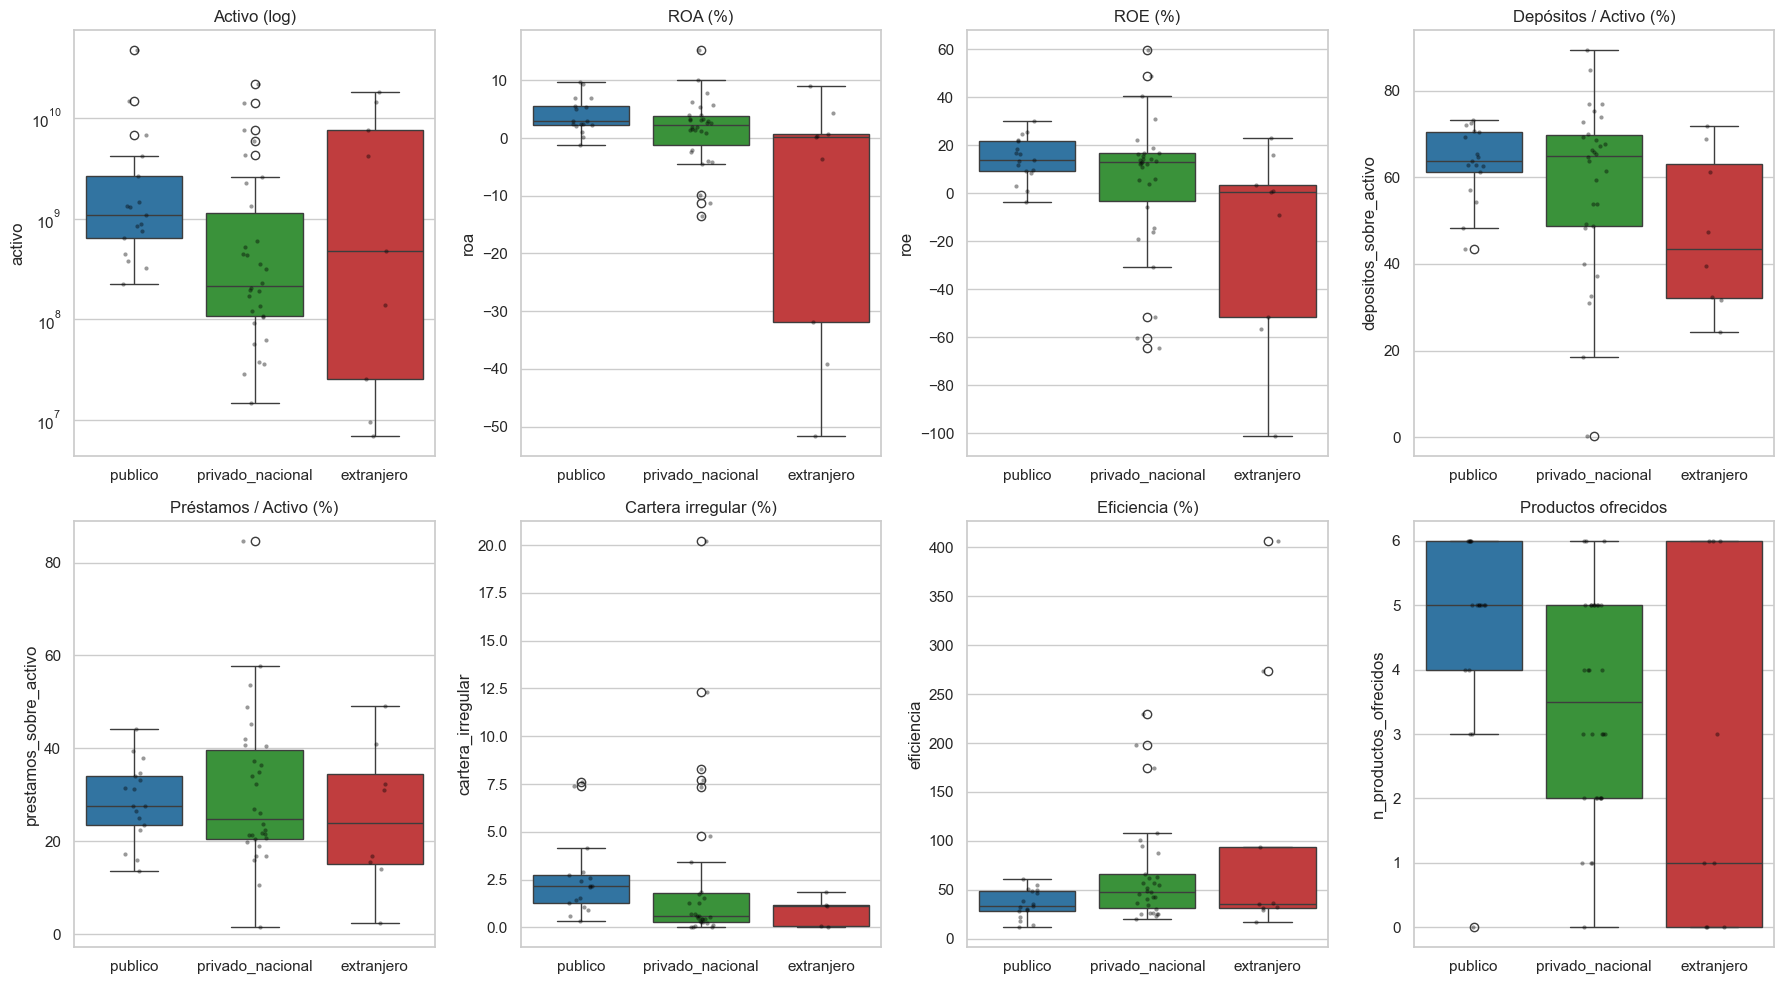
\includegraphics[width=\textwidth]{figs_entrega3/fig_eda_boxplots_tipo.png}
\caption{Distribución de ocho ratios por tipo de entidad (Dic-24). El fuerte solapamiento de las cajas
---incluso en los ratios estadísticamente significativos--- muestra que el tipo administrativo no separa
nítidamente los perfiles económicos. La escala del activo se grafica en escala logarítmica.}
\label{fig:boxplots}
\end{figure}

\paragraph{Dinámica temporal.} Entre Dic-23 y Dic-25, el ROA mediano cae fuerte en los tres tipos de
entidad, pasando de 4,15 a 0,79 en los públicos y de 3,06 a 0,35 en los privados nacionales, lo cual es
consistente con el fin del ciclo de LELIQ \citep{bcra2024ief}. En el mismo período, la cartera irregular
se duplica en los públicos, pasando de 2,33 a 5,05, y casi se duplica en los privados, pasando de 1,85 a
3,38. A su vez, el ratio préstamos/activo sube de aproximadamente 14\,\% a aproximadamente 38\,\% en los
privados nacionales, una señal de reactivación del crédito que todavía no se traduce en mayor
rentabilidad. Esta dinámica motiva modelar sobre el promedio de los tres cortes, entendido como un
perfil estructural estable, y dejar el análisis de las transiciones año a año como una extensión futura
del trabajo.

\paragraph{Oferta comercial.} La oferta de productos aporta información que el balance no refleja
(Figura~\ref{fig:oferta}). Los privados nacionales se especializan en plazo fijo, con una mediana de
11 variantes, y prácticamente no ofrecen hipotecas ni prendarios. Los públicos, en cambio, tienen la
oferta más balanceada entre categorías y son los únicos con presencia significativa en paquetes,
con una mediana de 3,5, y en hipotecas. Los extranjeros muestran una oferta diversificada pero acotada
en cada categoría individual, lo cual es consistente con un foco comercial en segmentos de altos
ingresos. Estas asimetrías son sustantivas: no derivan del tamaño de las entidades ni de su
rentabilidad, sino de decisiones de estrategia comercial, y son la razón por la cual incorporar la
oferta al conjunto de variables permite, como se verá más adelante, separar perfiles que el balance
por sí solo confunde.

\begin{figure}[htbp]
\centering
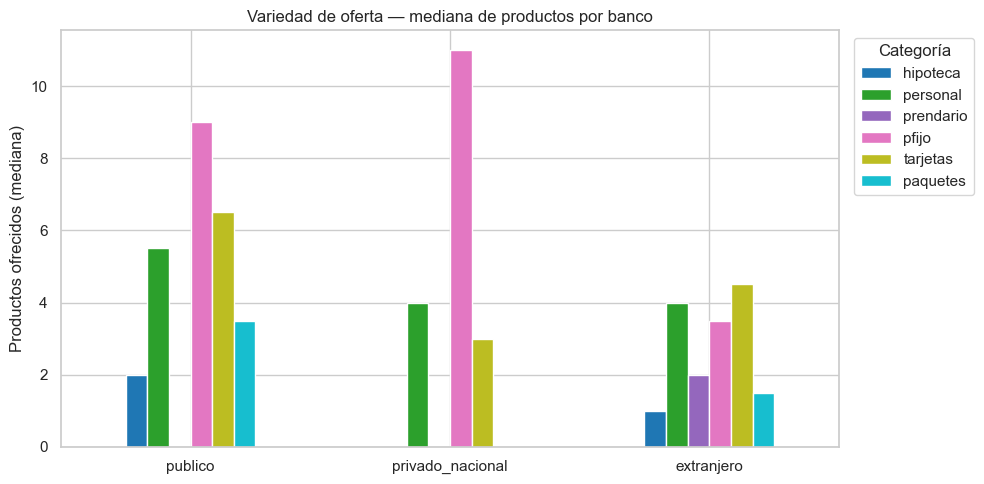
\includegraphics[width=0.85\textwidth]{figs_entrega3/fig_eda_oferta.png}
\caption{Variedad de oferta comercial: mediana de productos ofrecidos por banco en cada categoría, según
tipo de entidad (Régimen de Transparencia). Los privados nacionales concentran su oferta en plazo fijo; los
públicos son los más balanceados y los únicos con paquetes e hipotecas relevantes; los extranjeros
diversifican pero con baja profundidad por categoría.}
\label{fig:oferta}
\end{figure}

\subsection{Técnicas de análisis y modelado}
\label{sec:tecnicas}

\paragraph{Universo de modelado.} Se trabaja con \textbf{52 bancos} (los 56 menos los 4 mayoristas sin
cartera minorista: Bank of China, JPMorgan, BNP Paribas, Cetelem, cuyas métricas retail no aplican). El
\textit{dataset} de modelado es el promedio de los tres cortes por banco.

\paragraph{Espacio de variables (21).} Un espacio mixto que integra balance y oferta:
\begin{itemize}
  \item \textbf{10 variables continuas:} logaritmo del activo, préstamos/activo, títulos/activo,
  depósitos/activo, patrimonio/activo, ROA, liquidez, eficiencia, cartera irregular y logaritmo del
  activo por empleado. Sobre las variables más sesgadas (liquidez, cartera irregular y eficiencia) se
  aplica una transformación logarítmica, y luego todas se escalan con un método robusto a valores
  extremos (\textit{RobustScaler}), apropiado dada la dispersión del sistema.
  \item \textbf{11 binarias de oferta:} disponibilidad de caja de ahorro (pesos/USD), cuenta corriente,
  plazo fijo, tarjeta de crédito/débito, préstamo personal/hipotecario/prendario, paquete, segmento
  premium, entre otras. Concatenadas sin escalar, con peso 1,0.
\end{itemize}

\paragraph{Reducción dimensional (PCA).} Se utilizó para diagnóstico y visualización. En el espacio mixto de variables, los dos primeros
componentes principales explican en conjunto el 54\,\% de la varianza total (Figura~\ref{fig:pca}).
Para explicar el 80\,\% de la varianza se necesitan 5 componentes, y para explicar el 90\,\% se
necesitan 8. Esto confirma que la heterogeneidad entre bancos es genuinamente multidimensional, es
decir, no puede resumirse en un único eje que represente simplemente el tamaño de la entidad.

\begin{figure}[htbp]
\centering
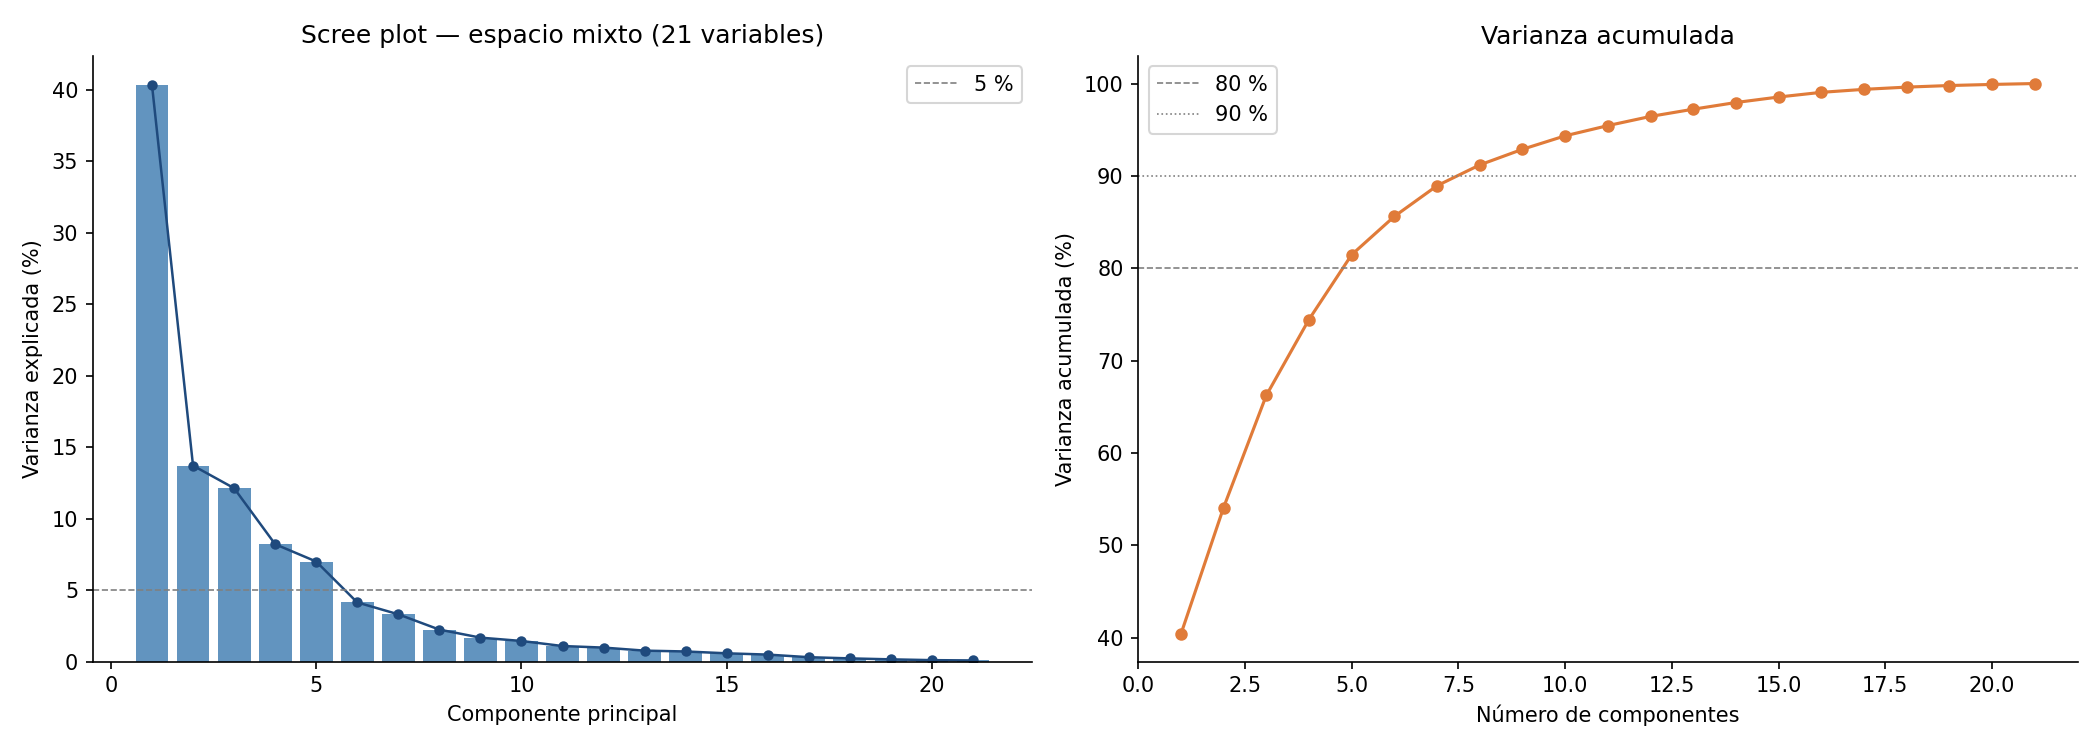
\includegraphics[width=0.95\textwidth]{figs_entrega3/fig_pca_scree.png}
\caption{\textit{Scree plot} (izq.) y varianza acumulada (der.) del PCA sobre el espacio mixto de 21
variables del modelo principal. Los dos primeros componentes explican el 54\,\% de la varianza; el 80\,\%
se alcanza con 5 componentes y el 90\,\% con 8: la caída es gradual y el sistema no se resume en pocos
ejes dominantes.}
\label{fig:pca}
\end{figure}
\paragraph{Comparación sistemática de modelos.} Se exploraron y compararon varias combinaciones de
espacio de variables y algoritmo de \textit{clustering}:
\begin{itemize}
  \item \textbf{K-Means $k=3$} sobre las 21 variables originales, con estandarización mediante
  StandardScaler (modelo base de comparación).
  \item \textbf{GMM $k=3$} sobre las 10 variables continuas de balance, aplicando transformación
  logarítmica y RobustScaler, sin incluir la oferta comercial.
  \item \textbf{GMM $k=3$ sobre el espacio mixto} de variables de balance y oferta comercial, probado
  en dos variantes que difieren en la ponderación asignada a las variables binarias de oferta
  (peso 1,0 y peso 0,5).
  \item \textbf{Contrastes con otros algoritmos:} se aplicaron también \textit{clustering} jerárquico
  de Ward y DBSCAN, basado en densidad, con el fin de verificar que la partición obtenida no sea un
  artefacto propio del algoritmo elegido, sino que se sostenga bajo distintos enfoques.
\end{itemize}
El número de \textit{clusters} se seleccionó combinando tres criterios, el coeficiente de
\textit{silhouette}, el índice de Davies-Bouldin y el método del codo, los cuales coinciden de forma
robusta en $k=3$ para todos los modelos evaluados. La elección del modelo final no se basa únicamente
en estos criterios cuantitativos, sino que combina la interpretabilidad sustantiva de los grupos
obtenidos con los resultados de la validación supervisada, que se describe a continuación
(Sección~\ref{sec:discusion}).

\paragraph{Validación supervisada.} Para verificar que los grupos identificados no sean un artefacto
del algoritmo de \textit{clustering}, se entrena un clasificador LightGBM multiclase sobre las
etiquetas obtenidas, utilizando como \textit{inputs} las variables originales. La lógica es la
siguiente: si un modelo supervisado, independiente del algoritmo de \textit{clustering}, logra
predecir esas etiquetas con buena performance, esto indica que la partición refleja una estructura
real presente en los datos y no un ordenamiento arbitrario. Para estimar la capacidad de
generalización del modelo con un tamaño muestral reducido, se emplea \textbf{validación cruzada
anidada}, con 5 particiones externas y 3 internas. Dentro del ciclo interno se realiza una
\textbf{búsqueda aleatoria de hiperparámetros} de 30 iteraciones, optimizando la métrica macro-F1 en
lugar de la \textit{accuracy}, dado el desbalance existente entre las clases (27, 15 y 10 observaciones,
respectivamente). Adicionalmente, se aplica \textbf{ponderación de clases} mediante la opción
\texttt{class\_weight} balanceada, con el objetivo de compensar ese mismo desbalance durante el
entrenamiento.

\paragraph{Interpretabilidad (SHAP).} Sobre el modelo final se calculan valores SHAP, tanto a nivel
global, para estimar la importancia de cada variable en el conjunto del modelo, como a nivel de cada
clase individual, para identificar qué variables definen a cada perfil y con qué peso relativo
contribuyen a esa definición.

\subsection{Selección de características}
\label{sec:seleccion}

El diseño de variables retoma el esquema \textit{choice/outcome} de \citet{roengpitya2014}, pero lo
adapta a las particularidades del caso. En el esquema original, las variables de resultado (ROA,
eficiencia, cartera irregular) se reservan para describir los grupos \textit{a posteriori}. En este trabajo,
en cambio, esas tres variables sí integran el espacio de \textit{clustering} junto con las de
elección (estructura de balance y oferta comercial), porque sin ellas el algoritmo no separa los tres
modelos de negocio de forma interpretable: el sistema argentino presenta gradientes entre perfiles que las
variables de balance ``puro'' no alcanzan a resolver. Se excluye ROE del espacio de \textit{clustering} por
su alta colinealidad con ROA ($\rho = 0{,}92$), y se lo conserva como variable puramente descriptiva.

Esta adaptación metodológica introduce un riesgo de circularidad, definir grupos con variables que luego
los explican, que se controla \textit{ex post}: la validación supervisada (Sección~\ref{sec:res2}) opera
solo sobre las etiquetas resultantes, sin acceso al proceso de \textit{clustering}, de modo que su alta
\textit{accuracy} constituye evidencia independiente de que la partición es real y no un mero reflejo de
las variables elegidas. Respecto de la ponderación de las binarias de oferta, se evaluaron dos pesos (1,0
y 0,5): el peso 1,0 maximiza la interpretabilidad y la coincidencia con el modelo base. Finalmente, las
binarias casi constantes en el panel (plazo fijo, prendario) resultan sin poder discriminante, como
confirma el análisis SHAP.

\subsection{Métricas de evaluación}

\begin{itemize}
  \item \textbf{Internas (\textit{clustering}):} \textit{silhouette} y Davies-Bouldin (calidad geométrica),
  Adjusted Rand Index (ARI) y NMI (coincidencia entre particiones).
  \item \textbf{Supervisadas (validación):} \textit{accuracy} y macro-F1 (esta última como métrica primaria,
  por el desbalance de clases), con \textit{precision}/\textit{recall}/F1 por clase.
\end{itemize}
Las métricas internas se utilizan para seleccionar el valor de $k$, mientras que la elección del
modelo final se argumenta combinando las métricas de validación supervisada con la interpretabilidad
de los grupos obtenidos (Sección~\ref{sec:discusion}).

\subsection{Métodos estadísticos}

Se emplean el test de Kruskal-Wallis (no paramétrico) para contrastar igualdad de distribuciones
de ratios entre tipos de entidad; la validación cruzada anidada (5$\times$3) con búsqueda aleatoria
de hiperparámetros para estimar la generalización; y los valores SHAP para la atribución de
importancia por variable y por clase.

% ============================================================
\section{Resultados y discusión}
\label{sec:resultados}
% ============================================================

\subsection{Segmentación no supervisada}
\label{sec:res1}

El modelo principal es el GMM con $k=3$, aplicado sobre el espacio mixto de
variables (balance y oferta comercial) y con un peso de 1,0 para las variables binarias de oferta.
Este modelo produce una partición de 27, 15 y 10 bancos, respectivamente, que se corresponde de forma
clara con tres modelos de negocio reconocibles (Figura~\ref{fig:pca_clusters}). Cabe aclarar que existen
alternativas con un valor de \textit{silhouette} más alto; la razón por la cual se elige este modelo por
sobre esas alternativas se argumenta en detalle en la Sección~\ref{sec:discusion}.

\begin{figure}[htbp]
\centering
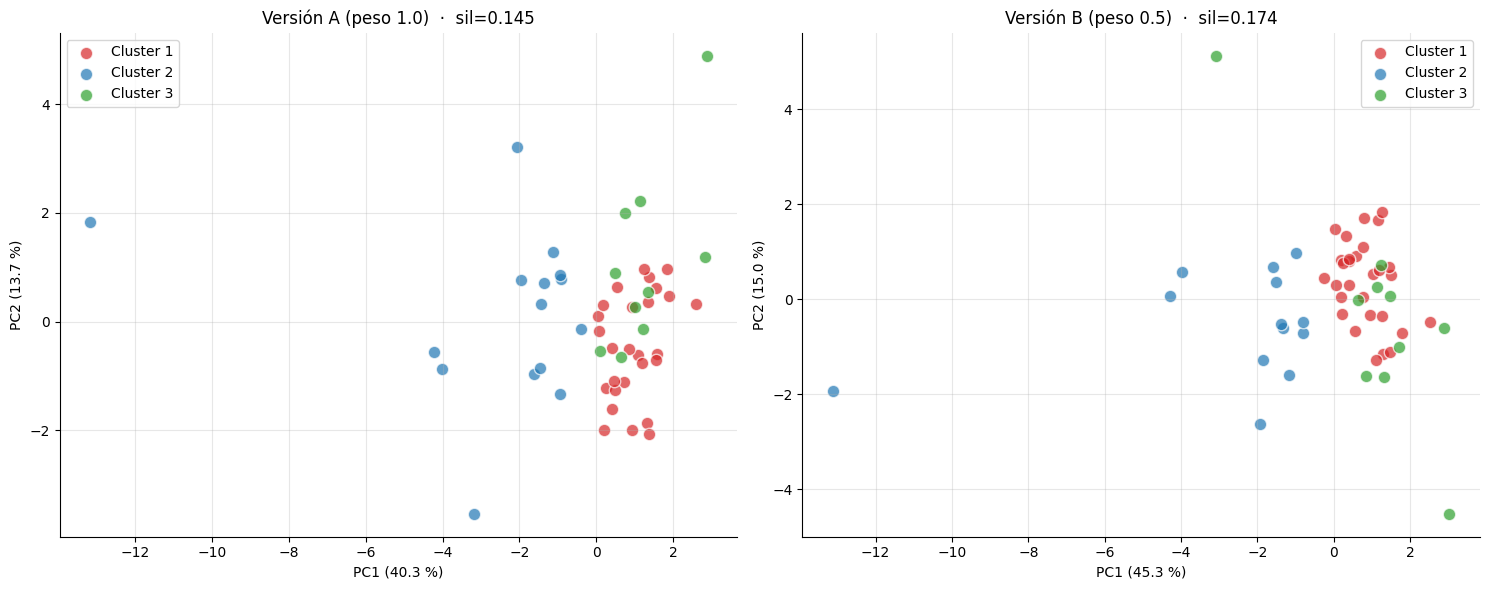
\includegraphics[width=0.95\textwidth]{figs_entrega3/fig_clustering_pca.png}
\caption{Proyección PCA (PC1 40,3\,\% $\cdot$ PC2 13,7\,\%) de los 52 bancos coloreada por \textit{cluster}
del modelo GMM sobre el espacio mixto. El panel izquierdo corresponde al modelo elegido (peso de las
binarias 1,0, \textit{silhouette} 0,145); el derecho, a la variante con peso 0,5 (\textit{silhouette}
0,174), descartada por su menor coincidencia con el modelo base y menor interpretabilidad
(Sección~\ref{sec:seleccion}). En ambos casos la nube es continua, sin separaciones nítidas entre grupos:
las fronteras entre perfiles son difusas, lo que el \textit{silhouette} refleja y la validación supervisada
explica como solapamiento entre perfiles, no como una falla del modelo.}
\label{fig:pca_clusters}
\end{figure}

\paragraph{Cluster 0: Banca universal masiva (27 bancos).}
El perfil mediano de este grupo presenta un ROA de 3,1\,\%, depósitos que representan el 66\,\% del
activo, una eficiencia de 43\,\% y una oferta retail completa (paquetes premium 67\,\%, hipotecas 78\,\%,
tarjetas premium 59\,\%). Es el núcleo del sistema bancario tradicional: incluye a Galicia, Nación, BBVA,
Santander, todos los públicos provinciales, Macro, Patagonia, Supervielle y Credicoop. Representa el
modelo de \textbf{banca universal}, es decir, entidades grandes, con red de sucursales, que se fondean
principalmente con depósitos del sector privado y que ofrecen la gama completa de productos, desde la
caja de ahorro hasta el crédito hipotecario y los paquetes premium, combinando negocio minorista y
mayorista. Su rentabilidad positiva y su eficiencia razonable reflejan las economías de escala propias
de este tipo de entidades. Lo más relevante de este cluster es su composición: reúne bajo un mismo
modelo de negocio a bancos públicos provinciales y a grandes bancos privados y extranjeros, entidades
que la clasificación administrativa separa pero que en la práctica operan de forma equivalente. Esto
constituye la evidencia más directa de que el modelo de negocio, y no el tipo de propiedad, es el eje
que estructura el sistema.

\paragraph{Cluster 1: Banca minorista en transformación (15 bancos).}
El perfil mediano de este grupo presenta un ROA de $-2{,}3$\,\%, siendo el único cluster con rentabilidad
negativa; una eficiencia de 80\,\%, que indica un \textit{cost-to-income} deteriorado; y una cartera
irregular de 4,3\,\%. Estos bancos ofrecen préstamos personales en un 87\,\% de los casos, pero casi no
ofrecen hipotecas (20\,\%). Se trata del cluster más heterogéneo en apariencia, aunque coherente en su
lógica interna: agrupa a los 4 bancos 100\,\% digitales (Brubank, Ualá, Voii, Dino), a entidades de
\textit{consumer finance} (Servicios Financieros, Columbia, Sucrédito, Masventas) y a privados chicos con
dificultades (Banco Meridian, Banco Julio, Banco Piano). Lo que une a estas entidades, más allá de sus
diferencias superficiales, es un modelo común de banca minorista de nicho o en construcción:
un foco en el crédito al consumo, una escala insuficiente para diluir costos fijos, y una rentabilidad
todavía negativa. Esta rentabilidad negativa responde a causas distintas según el sub-grupo: en el caso
de los bancos digitales, refleja una etapa de inversión activa para crecer; en el caso de los bancos
tradicionales chicos, refleja un negocio estructuralmente más difícil de sostener. Por este motivo, el
sub-perfil \textit{fintech} se incluye dentro de este cluster y no como una clase separada: comparte con
el resto del grupo el rasgo central de rentabilidad débil y foco en el consumo, aun cuando el origen de
esa debilidad sea diferente. Desde una óptica de supervisión bancaria, este es el grupo que requiere
seguimiento prioritario.

\paragraph{Cluster 2: Banca corporativa y de mercado de capitales (10 bancos).}
El perfil mediano de este grupo presenta un ROA de 3,2\,\%, una eficiencia de 30\,\% (la más baja del
sistema, es decir, la mejor), depósitos que representan solo el 45\,\% del activo, y una cartera
irregular de apenas 0,6\,\% (morosidad casi nula). Estas entidades casi no ofrecen productos minoristas:
hipotecas en un 10\,\% de los casos y paquetes en otro 10\,\%. El grupo reúne a Citibank, Banco de
Valores, Mariva, BICE, CMF y BACS, y corresponde al modelo de banca corporativa y de mercado de
capitales. Estas entidades se fondean en el mercado mayorista o con capital propio, en lugar de
depender del depósito minorista, e invierten o titulizan en lugar de prestar a familias. Su morosidad
casi nula no refleja una mejor gestión del riesgo minorista, sino directamente la ausencia de ese
riesgo: al no tener prácticamente cartera de consumo, no están expuestas a ese tipo de incumplimientos.
Este es el perfil que el modelo caracteriza tanto por lo que hace (invertir, operar en el mercado de
capitales) como por lo que no hace (captar depósitos minoristas, ofrecer productos masivos), y es el
que más se aproxima a la categoría de ``banca de inversión'' dentro de la tipología de
\citet{roengpitya2014}.

\subsubsection{Hallazgos estructurales}

\begin{itemize}
  \item \textbf{El tipo de entidad no segmenta.} Públicos provinciales y privados grandes comparten el
  \textit{cluster} minorista cuando comparten modelo de negocio. La propiedad (público/privado/extranjero)
  no es el eje de segmentación; el modelo de negocio sí. Esto verifica el primer sentido operativo de la
  hipótesis general (Sección~\ref{sec:objetivos}).
  \item \textbf{El sub-grupo digital queda identificado.} Los 4 digitales caen juntos en ``Chicos en
  transformación'', sin dispersarse entre perfiles.
\end{itemize}

\paragraph{Modelos de contraste.} La comparación sistemática entre modelos (Cuadro~\ref{tab:modelos})
no solo justifica la elección del modelo final, sino que aporta evidencia adicional sobre la naturaleza
del sistema bancario argentino:
\begin{itemize}
  \item \textbf{K-Means} logra un \textit{silhouette} de 0,243 y separa tres perfiles de balance
  claramente diferenciados, pero dispersa a los 4 bancos digitales entre los tres \textit{clusters},
  sin lograr identificarlos como un grupo diferenciado: la dimensión \textit{fintech} directamente no
  emerge con este modelo.
  \item \textbf{GMM sobre variables continuas solamente} es el primer modelo que logra agrupar a los
  bancos digitales en un mismo cluster, pero, al descartar la oferta comercial, pierde la distinción
  entre banca mayorista y minorista (el índice ARI contra el modelo base es de apenas 0,215, lo que
  indica que se trata de una partición esencialmente distinta, no de una versión mejorada de la misma).
  \item \textbf{GMM sobre el espacio mixto} logra recuperar ambas ventajas simultáneamente: agrupa
  correctamente a los bancos digitales y, al mismo tiempo, restaura la distinción entre los tres modelos
  de negocio. Es, además, el modelo con el ARI más alto respecto del modelo base (0,594), lo cual indica
  que es la versión que mejor conserva la intuición original de K-Means, a la vez que mejora la
  precisión de sus fronteras entre grupos.
  \item \textbf{Ward y DBSCAN} confirman que la estructura del sistema no es de naturaleza jerárquica ni
  densa. El coeficiente cofenético de Ward es de 0,457, lo que indica que no existen subgrupos limpios
  anidados dentro de la estructura jerárquica. Por su parte, DBSCAN clasifica al 84\,\% de los bancos
  como ruido, y solo logra formar regiones densas entre los bancos minoristas de mayor tamaño. En
  conjunto, todos los algoritmos coinciden en identificar el mismo ``esqueleto'' general del sistema
  (los bancos minoristas grandes por un lado, y el resto por otro), pero difieren en la definición
  precisa de las fronteras finas entre grupos. Esto constituye evidencia de que los perfiles bancarios
  se solapan genuinamente en sus zonas de frontera, y no de una falla propia de un método en particular.
\end{itemize}

\begin{table}[htbp]
\centering
\caption{Comparación sistemática de modelos de \textit{clustering}. El modelo elegido (en negrita) no es el
de mayor \textit{silhouette}, pero es el único que agrupa los digitales sin perder la distinción
mayorista/minorista, y el de mayor coincidencia con el modelo base.}
\label{tab:modelos}
\small
\begin{tabular}{llrcr}
\toprule
\textbf{Modelo} & \textbf{Espacio} & \textbf{Silhouette} & \textbf{Digitales agrup.} & \textbf{ARI vs.\ K-Means} \\
\midrule
K-Means $k=3$ & 21 feat + StandardScaler & 0,243 & No (dispersos) & --- \\
GMM $k=3$ & 10 continuas + log & 0,262 & Sí & 0,215 \\
\textbf{GMM $k=3$} & \textbf{mixto (peso 1,0)} & \textbf{0,145} & \textbf{Sí (anidados)} & \textbf{0,594} \\
GMM $k=3$ & mixto (peso 0,5) & 0,174 & Sí & 0,427 \\
\bottomrule
\end{tabular}
\end{table}

\subsection{Validación supervisada e interpretabilidad}
\label{sec:res2}

Un clasificador supervisado independiente aprende a reproducir las etiquetas del \textit{clustering} a
partir de las variables originales. Esta etapa permite determinar si la partición es predecible y
coherente, o si, por el contrario, constituye un artefacto del algoritmo, lo cual corresponde al segundo
sentido en el que se contrasta la hipótesis general.

\paragraph{Desempeño en validación externa.} El modelo alcanza una \textit{accuracy} de $0{,}867 \pm 0{,}075$
y un macro-F1 de $0{,}850 \pm 0{,}081$. Al desagregar por clase, los valores de F1 se ubican entre 0,83 y
0,89, lo que indica que el desbalance entre clases (27/15/10 observaciones) no degrada el desempeño en las
clases más chicas. Para un tamaño muestral de $n = 52$ evaluado con validación cruzada anidada, una
\textit{accuracy} de 0,87 constituye un valor alto, por encima de lo que se esperaría de una partición
arbitraria o de un clasificador que acertara por azar. La matriz de confusión (Figura~\ref{fig:confusion})
concentra 45 de los 52 bancos sobre la diagonal principal, es decir, correctamente clasificados en su
cluster de origen.

\begin{figure}[htbp]
\centering
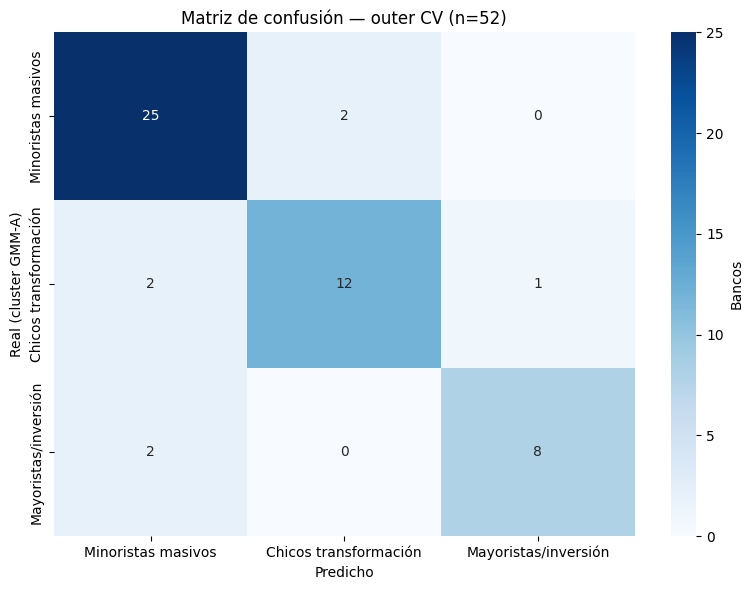
\includegraphics[width=0.7\textwidth]{figs_entrega3/fig_matriz_confusion.png}
\caption{Matriz de confusión (validación cruzada anidada, $n = 52$). La diagonal concentra 45 de 52 bancos.
Los 7 errores se ubican en las fronteras entre perfiles y nunca confunden perfiles opuestos: ningún
minorista típico se predice como mayorista.}
\label{fig:confusion}
\end{figure}
\paragraph{Los errores se concentran en las zonas de frontera entre perfiles.} Los 7 errores de
clasificación no corresponden a casos típicos de cada grupo, sino a entidades con perfiles ambiguos o
de transición: BROU (un \textit{outlier} extremo, con ROA de $-35$\,\% y eficiencia de 407\,\%), Columbia
y Dino (entidades ambiguas entre \textit{consumer finance} y modelo digital), Sgo.\ del Estero y Banco de
Comercio (en la frontera entre el perfil mayorista y el minorista), y Municipal Rosario y Coinag
(minoristas deteriorados, al borde de la transformación hacia otro perfil). El hecho de que los errores
se concentren justamente en los bancos a los que el GMM ya había asignado una probabilidad de pertenencia
baja confirma que el GMM y el clasificador LightGBM están captando el mismo continuo subyacente en los
datos, aunque cada uno lo segmenta en puntos ligeramente distintos.

\paragraph{Variables que definen cada perfil (SHAP).} El análisis global (Figura~\ref{fig:shap_global})
muestra que las variables con mayor peso en la definición de los perfiles son tres variables financieras,
ROA, cartera irregular y eficiencia, seguidas por dos variables comerciales, la oferta de paquetes y la
oferta de paquetes premium. La descomposición por clase (Figura~\ref{fig:shap_clase}) permite ir un paso
más allá y muestra que cada cluster tiene una combinación de variables propia, con escaso solapamiento
entre perfiles:
\begin{itemize}
  \item \textbf{Banca universal masiva:} este perfil se define principalmente por la oferta retail de
  tipo premium (oferta de paquetes, $|\text{SHAP}| = 1{,}57$; segmento premium, 1,36; hipotecas, 0,68) y,
  en segundo lugar, por la escala de la entidad (préstamos sobre activo, 1,15; logaritmo del activo, 0,49).
  En este caso, la variable con mayor poder discriminante proviene de la oferta comercial y no de las
  variables de balance.
  \item \textbf{Banca minorista en transformación:} este perfil se define casi por completo por la
  rentabilidad y la eficiencia de las entidades, en particular por un ROA negativo
  ($|\text{SHAP}| = 3{,}30$) y una eficiencia deteriorada (1,43), mientras que las variables de oferta
  de productos prácticamente no contribuyen a distinguir a este grupo.
  \item \textbf{Banca corporativa y de mercado de capitales:} este perfil se define por una morosidad
  baja (cartera irregular reducida, $|\text{SHAP}| = 2{,}39$), una eficiencia muy baja, entendida aquí
  como un \textit{cost-to-income} bajo y típico de la banca corporativa, y una proporción baja de
  préstamos sobre el activo total. A diferencia de los otros dos perfiles, este cluster queda
  caracterizado tanto por la presencia de ciertos rasgos financieros como por la ausencia de rasgos
  comerciales minoristas.
\end{itemize}

\begin{figure}[htbp]
\centering
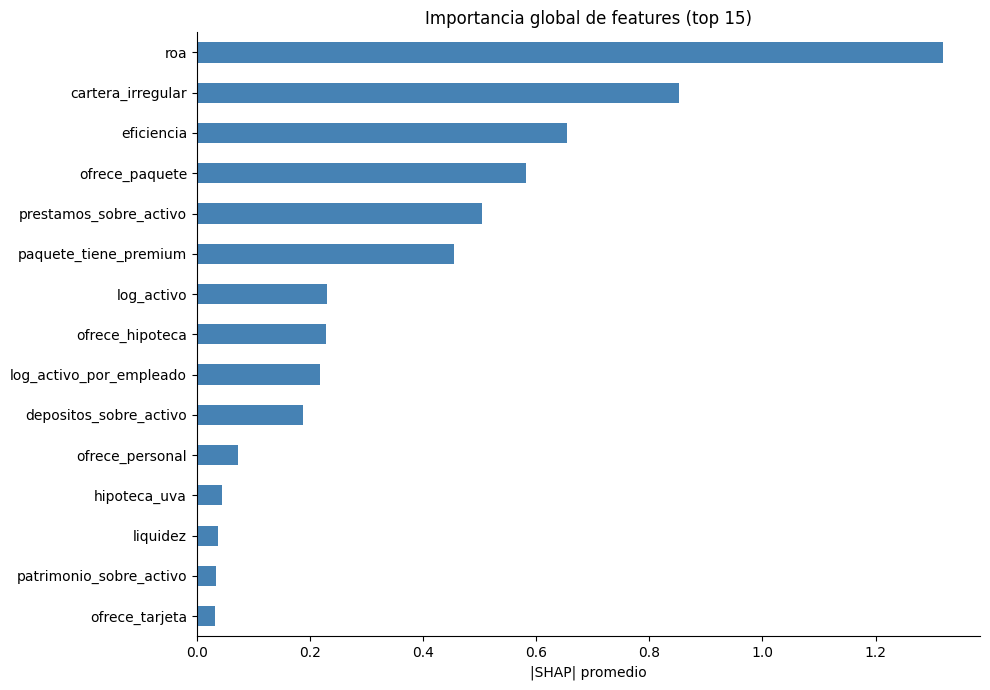
\includegraphics[width=0.9\textwidth]{figs_entrega3/fig_shap_global.png}
\caption{Importancia global SHAP ($|\text{SHAP}|$ promedio, top 15). Dominan tres variables financieras
---ROA, cartera irregular y eficiencia--- seguidas de dos comerciales: la oferta de paquetes y la de
paquetes premium. Las binarias casi constantes (plazo fijo, prendario) no aportan.}
\label{fig:shap_global}
\end{figure}

\begin{figure}[htbp]
\centering
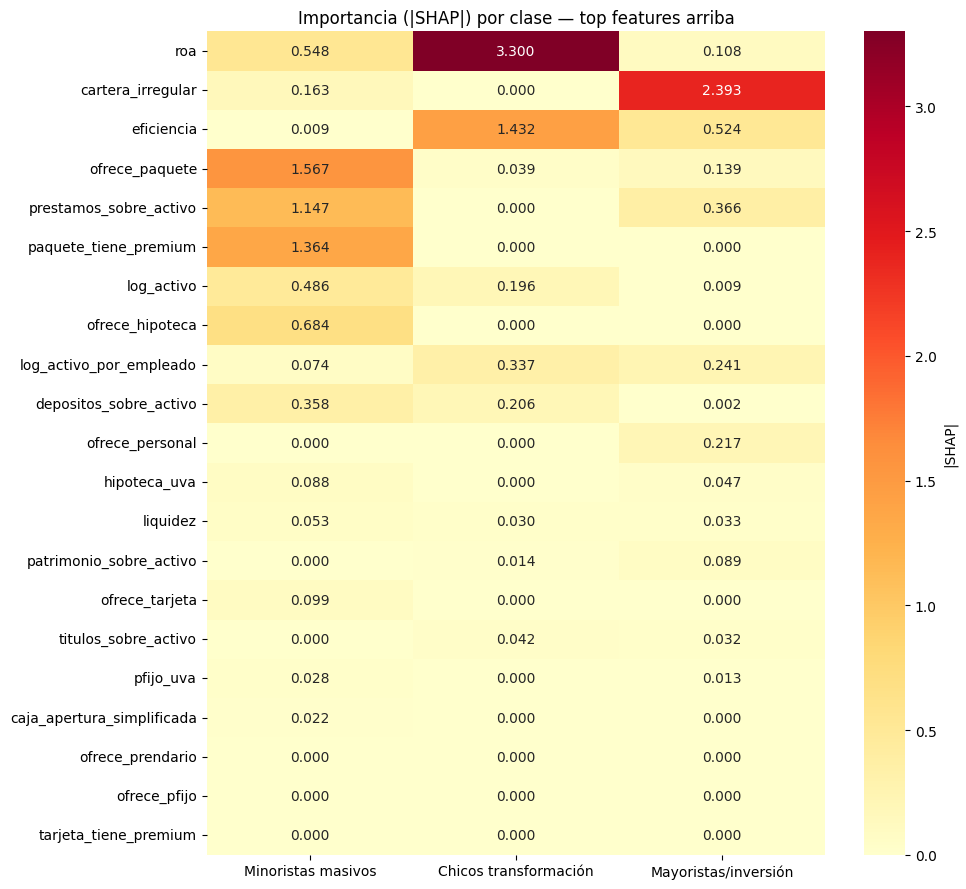
\includegraphics[width=0.9\textwidth]{figs_entrega3/fig_shap_por_clase.png}
\caption{Importancia SHAP descompuesta por clase. Cada \textit{cluster} presenta un conjunto de variables
determinantes distinto y con escaso solapamiento: el ROA define a la banca minorista en transformación, la baja
morosidad a los mayoristas, y la oferta retail premium a la banca universal masiva.}
\label{fig:shap_clase}
\end{figure}

\paragraph{Coherencia con la segmentación.} El análisis SHAP recupera las mismas variables con que se había
caracterizado cada perfil ---ROA, cartera irregular, eficiencia, paquetes premium e hipotecas--- sin haberlas
recibido como entrada explícita para esa tarea. La interpretación del \textit{clustering} y la del
clasificador convergen de forma independiente.

\paragraph{Alcance de la validación.} El clasificador no demuestra que $k=3$ sea el número óptimo de grupos
ni que el modelo elegido supere en términos absolutos a las demás particiones; confirma que, dada esa
partición, es coherente y reproducible a partir de las variables. Tampoco aísla la dimensión digital como
clase propia: las entidades digitales quedan comprendidas dentro del cluster ``Banca minorista en transformación''.

\subsection{Discusión de los resultados y su relevancia}
\label{sec:discusion}
El hallazgo central del trabajo es la coexistencia de un \textit{silhouette} bajo (0,145) con una
\textit{accuracy} de validación alta (0,867). Esta combinación constituye el resultado más relevante del
análisis y requiere una interpretación cuidadosa.
\begin{itemize}
  \item \textbf{El \textit{silhouette} bajo aporta información sobre la estructura del sistema.} El
  \textit{silhouette} mide la compacidad geométrica de los grupos. En un espacio donde los perfiles se
  diferencian por combinaciones de variables, y no por una única variable que los separe nítidamente, y
  donde además existen bancos ubicados en zonas de frontera entre perfiles, cualquier partición discreta
  tenderá a arrojar un \textit{silhouette} bajo. El valor observado refleja límites difusos entre los
  grupos, más que la calidad del agrupamiento en sí.
  \item \textbf{La validación triangula la calidad de la partición.} El \textit{silhouette} bajo se
  contrapesa con tres evidencias independientes que apuntan en la misma dirección: una \textit{accuracy}
  de 0,867 en validación cruzada anidada, una atribución SHAP coherente con los perfiles definidos, y un
  ARI de 0,594 respecto del modelo base de K-Means. En conjunto, estas evidencias indican que la
  partición es real, aunque con fronteras difusas entre grupos.
  \item \textbf{Elección del modelo.} La decisión se basa en la interpretabilidad de los perfiles y en la
  validación supervisada, y no exclusivamente en la métrica geométrica. Este criterio es consistente con
  \citet{mercadier2025}, para quienes el \textit{silhouette} y el índice de Davies-Bouldin funcionan como
  indicadores complementarios dentro de un análisis más amplio, y no como un veredicto único y suficiente
  por sí mismo.
\end{itemize}

\paragraph{Implicancia macroprudencial.}
El hallazgo de que el tipo administrativo no segmenta el sistema tiene una lectura regulatoria concreta.
La supervisión bancaria suele organizarse, implícita o explícitamente, en torno a categorías
administrativas: bancos públicos, privados nacionales y extranjeros. Sin embargo, los resultados
sugieren que esa partición no se corresponde necesariamente con la exposición real al riesgo. Por
ejemplo, un banco público provincial minorista y un gran banco privado comparten un mismo perfil de
riesgo (Cluster 0), pese a tener distinta propiedad. Al mismo tiempo, dos entidades igualmente
clasificadas como ``privadas nacionales'' pueden pertenecer a clusters opuestos: una puede ser banca
minorista masiva, y la otra, banca minorista de nicho en pérdida. Una supervisión organizada en torno al
modelo de negocio, en lugar de la forma administrativa, podría captar de forma más precisa dónde se
concentran las vulnerabilidades del sistema.

En esa línea, el trabajo ofrece un mapa posible. El Cluster 1 (Banca minorista en
transformación) combina ROA negativo con eficiencia deteriorada. Por eso aparece como el grupo de
seguimiento prioritario, ya que combina rentabilidad negativa con escala insuficiente. Dentro de este
grupo, el sub-grupo digital merece una atención particular, ya que es emergente y está en rápida
expansión. Un seguimiento específico de estas entidades permitiría distinguir dos tipos de pérdida: la
asociada a una etapa de inversión para crecer, y la asociada a un modelo de negocio poco viable.

La dinámica temporal documentada en el análisis exploratorio añade relevancia a este punto. En ese
análisis se observó una caída generalizada del ROA y un aumento de la morosidad. Esto sugiere que los
perfiles no son necesariamente estáticos: un banco puede migrar entre ellos con el tiempo. Esta
migración entre perfiles podría estudiarse a futuro utilizando las probabilidades de pertenencia que el
GMM calcula para cada banco, ya que estas permiten observar si un banco se va acercando gradualmente a
otro perfil con el paso del tiempo (Sección~\ref{sec:conclusion}).

\subsection{Limitaciones y posibles mejoras}
\begin{itemize}
  \item \textbf{Muestra chica ($n = 52$):} el desvío estándar de 0,075 obtenido en la validación cruzada
  anidada implica que el valor real de la \textit{accuracy} se ubica, con alta probabilidad, en un rango
  aproximado de entre 0,79 y 0,94. Esto muestra que la precisión de la estimación está acotada por el
  tamaño reducido de la muestra.
  \item \textbf{El promedio de los tres cortes temporales oculta parte de la dinámica documentada en el
  análisis exploratorio}, en particular la caída del ROA y el aumento de la morosidad observados entre
  Dic-23 y Dic-25. Al trabajar con el promedio, el modelo prioriza la estabilidad estructural del perfil
  por sobre su evolución en el tiempo. Una mejora posible es analizar las transiciones de perfil banco
  por banco entre cada corte, en lugar de trabajar únicamente con el promedio agregado.
  \item \textbf{Las variables de oferta comercial capturan únicamente la disponibilidad de un producto,
  no su volumen de colocación ni su precio.} Es decir, indican si un banco ofrece o no un determinado
  producto, pero no cuánto de ese producto coloca efectivamente ni en qué condiciones. Una mejora
  posible es incorporar tasas de interés y comisiones como variables continuas adicionales, en lugar de
  limitarse a variables binarias de disponibilidad.
  \item \textbf{El clasificador supervisado hereda los sesgos propios del \textit{clustering} original:}
  dado que se entrena sobre las etiquetas generadas por el GMM, reproduce también los eventuales errores
  de asignación del modelo de base, en lugar de corregirlos de forma independiente.
\end{itemize}

% ============================================================
\section{Conclusión}
\label{sec:conclusion}
% ============================================================

\subsection{Resumen de los hallazgos principales}
El trabajo identifica tres perfiles de negocio diferenciados en el sistema bancario argentino: banca
universal masiva (27 bancos), banca minorista en transformación (15 bancos, con un sub-grupo digital
emergente) y banca corporativa y de mercado de capitales (10 bancos). Con esto, el trabajo responde de
forma afirmativa a la pregunta de investigación: existen perfiles diferenciados dentro del sistema, y es
posible identificar las variables que los definen. El tipo administrativo de la entidad
(propiedad) no segmenta el sistema: lo que efectivamente agrupa a los bancos es su modelo de negocio, y
no su forma administrativa. Las variables que definen cada perfil resultan interpretables y coherentes
desde el punto de vista económico: la rentabilidad y la eficiencia separan a la banca minorista en
transformación; la baja morosidad y el bajo fondeo minorista separan a la banca corporativa y de mercado
de capitales; y la oferta retail premium junto con la escala separan a la banca universal masiva. Por
último, la partición resulta predecible (\textit{accuracy} de 0,867) a pesar de presentar un
\textit{silhouette} bajo, lo que indica fronteras difusas entre los grupos, pero una estructura
subyacente real.

\subsection{Conclusiones generales y su relación con los objetivos}

Se cumplen los objetivos planteados. Se construyó un \textit{dataset} integrado que combina información de balance y de oferta comercial pública; se describió la heterogeneidad
estructural del sistema y su dinámica temporal; se aplicaron y compararon múltiples algoritmos de
\textit{clustering}; se caracterizó cada perfil por sus dimensiones económicas; y se validó la partición con
un clasificador supervisado interpretado con SHAP. La hipótesis general de trabajo queda respaldada en sus dos
sentidos operativos: el tipo administrativo no estructura los grupos, y un clasificador independiente reproduce
la partición con alta \textit{accuracy}.

El principal aporte metodológico, frente a una literatura centrada en métricas internas, es la
estrategia de validación triple ---interpretabilidad sustantiva, clasificador supervisado
independiente y coherencia de la atribución SHAP--- que permite sostener la elección de un modelo con
\textit{silhouette} bajo pero con estructura demostrablemente real. Esta estrategia también habilita la
decisión metodológica de relajar el esquema \textit{choice/outcome} sin incurrir en circularidad.

\subsection{Recomendaciones para futuros trabajos}

\begin{itemize}
  \item \textbf{Transiciones temporales.} Usar las probabilidades de pertenencia
  del GMM y/o aplicar el clasificador a cada corte por separado para detectar migraciones de perfil y evaluar
  si la digitalización se acelera.
  \item \textbf{Oferta como variable continua.} Incorporar tasas y comisiones del Régimen de Transparencia, hoy
  representado solo por la disponibilidad binaria de cada producto.
  \item \textbf{Dimensión digital explícita.} Tratar el sub-grupo \textit{fintech} como eje propio del análisis
  si la digitalización se vuelve central a la pregunta de investigación.
\end{itemize}

% ============================================================
\clearpage
\section{Bibliografía}
% ============================================================

\subsection{Referencias citadas}

\begingroup
\renewcommand{\section}[2]{}
\begin{thebibliography}{9}

\bibitem[BCRA(2024)]{bcra2024ief}
Banco Central de la República Argentina (2024). \textit{Informe de Estabilidad Financiera --- Primer
semestre de 2024.} BCRA. \url{https://www.bcra.gob.ar/PublicacionesEstadisticas/Informe-estabilidad-financiera.asp}

\bibitem[Chherawala et al.(2025)]{chherawala2025}
Chherawala, T., Vaidya, A., \& Basu, S. (2025). \textit{Multidimensional surveillance of the Indian banking
system: A cluster approach.} Journal of Applied Economic Sciences, 20(2), 255--272.

\bibitem[Ke et al.(2017)]{lightgbm}
Ke, G., Meng, Q., Finley, T., Wang, T., Chen, W., Ma, W., Ye, Q., \& Liu, T.-Y. (2017). \textit{LightGBM: A
highly efficient gradient boosting decision tree.} Advances in Neural Information Processing Systems, 30.

\bibitem[Lundberg \& Lee(2017)]{lundberg2017}
Lundberg, S. M., \& Lee, S.-I. (2017). \textit{A unified approach to interpreting model predictions.} Advances
in Neural Information Processing Systems, 30.

\bibitem[Mercadier et al.(2025)]{mercadier2025}
Mercadier, M., Tarazi, A., Armand, P., \& Lardy, J.-P. (2025). \textit{Monitoring bank risk around the world
using unsupervised learning.} European Journal of Operational Research, 324(2), 590--615.

\bibitem[Pedregosa et al.(2011)]{scikit-learn}
Pedregosa, F., et al. (2011). \textit{Scikit-learn: Machine learning in Python.} Journal of Machine Learning
Research, 12, 2825--2830.

\bibitem[Roengpitya et al.(2014)]{roengpitya2014}
Roengpitya, R., Tarashev, N., \& Tsatsaronis, K. (2014). \textit{Bank business models.} BIS Quarterly Review,
December, 55--65.

\end{thebibliography}
\endgroup

\subsection{Fuentes de datos primarias}

\begin{itemize}
  \item BCRA --- Portal de Entidades Financieras (estados contables, situación de deudores, datos de estructura).
  \item BCRA --- Régimen de Transparencia, Sección 36 (información comercial de productos).
  \item BCRA --- Comunicación ``A'' (clasificación de deudores: situaciones 1 a 5).
\end{itemize}

% ============================================================
\section{Anexos}
\label{sec:anexos}
% ============================================================

\subsection{Código fuente y reproducibilidad}

El código fuente completo ---el \textit{script} de \textit{scraping} y los notebooks del análisis (ingesta y
calidad, análisis exploratorio, \textit{clustering} base, alternativo y principal, y validación supervisada)---
está disponible en el repositorio público del proyecto. El repositorio incluye el archivo de dependencias
(\texttt{requirements.txt}) con las versiones de las bibliotecas utilizadas y las instrucciones para reproducir
el análisis de punta a punta.

\begin{notebox}
\small
\textbf{Repositorio:} \url{https://github.com/missvico/tesis-perfiles-bancarios}\\
\textbf{Software:} Python 3, con \texttt{scikit-learn}, \texttt{lightgbm}, \texttt{shap}, \texttt{pandas},
\texttt{numpy}, \texttt{scipy}, \texttt{matplotlib} y \texttt{seaborn} (versiones en \texttt{requirements.txt}).\\
\textbf{Datos:} el repositorio incluye la base de datos scrapeada del Portal de Entidades Financieras
y del Régimen de Transparencia, junto con el panel transversal consolidado (168 observaciones)
utilizado como base del análisis.\\
\textbf{Material complementario:} se incluyen además resúmenes en prosa por etapa del análisis
(\texttt{resumen\_eda.md}, \texttt{resumen\_clustering.md}, \texttt{resumen\_clustering\_alternativo.md}
y \texttt{resumen\_clasificador.md}), con tablas y figuras ampliadas que complementan las presentadas
en este documento.
\end{notebox}

\subsection{Glosario de términos técnicos}

\begin{description}
  \item[ARI (Adjusted Rand Index)] Métrica que mide el grado de coincidencia entre dos
  particiones de un mismo conjunto de datos, corregida por el acuerdo esperable al azar. Toma
  valor 1 cuando ambas particiones son idénticas y valores cercanos a 0 cuando la coincidencia
  no supera a la esperada de forma aleatoria.

  \item[Clustering] Conjunto de técnicas de aprendizaje no supervisado cuyo objetivo es agrupar
  observaciones similares entre sí, sin utilizar etiquetas previamente definidas.

  \item[Cost-to-income] Indicador de eficiencia que expresa los gastos de administración como
  proporción del margen operativo. Un valor más bajo indica una mayor eficiencia en la gestión
  de costos.

  \item[Davies-Bouldin (índice de)] Métrica interna de calidad de un agrupamiento que compara
  la dispersión dentro de cada grupo con la separación entre grupos. Valores más bajos indican
  una mejor definición de los grupos.

  \item[DBSCAN] Algoritmo de agrupamiento basado en densidad, que identifica grupos como
  regiones densas de observaciones y clasifica como ruido a los puntos que quedan en zonas de
  baja densidad.

  \item[GMM (Gaussian Mixture Model)] Modelo probabilístico de agrupamiento que asume que los
  datos provienen de una mezcla de distribuciones normales, y asigna a cada observación una
  probabilidad de pertenencia a cada grupo, en lugar de una asignación rígida.

  \item[K-Means] Algoritmo de agrupamiento que divide las observaciones en un número fijo de
  grupos, minimizando la distancia de cada observación al centro de su grupo.

  \item[LightGBM] Algoritmo de aprendizaje supervisado basado en árboles de decisión y en la
  técnica de \textit{gradient boosting}, utilizado en este trabajo para validar la partición
  obtenida por el agrupamiento.

  \item[Macro-F1] Promedio del puntaje F1 calculado de forma independiente para cada clase.
  Al no ponderar por el tamaño de las clases, resulta apropiado como métrica principal cuando
  existe desbalance entre ellas.

  \item[NMI (Normalized Mutual Information)] Métrica que cuantifica la información compartida
  entre dos particiones, normalizada para tomar valores entre 0 y 1.

  \item[PCA (Análisis de Componentes Principales)] Técnica de reducción de dimensionalidad que
  transforma un conjunto de variables correlacionadas en un conjunto menor de componentes no
  correlacionados, reteniendo la mayor parte de la varianza original.

  \item[RobustScaler] Método de escalado de variables que utiliza la mediana y el rango
  intercuartílico, lo que lo hace menos sensible a la presencia de valores extremos que el
  escalado estándar.

  \item[ROA (Return on Assets)] Indicador de rentabilidad que expresa el resultado del período
  como proporción del activo total de la entidad.

  \item[ROE (Return on Equity)] Indicador de rentabilidad que expresa el resultado del período
  como proporción del patrimonio neto de la entidad.

  \item[SHAP (SHapley Additive exPlanations)] Método de interpretabilidad que asigna a cada
  variable una contribución al resultado de un modelo, a partir de los valores de Shapley de la
  teoría de juegos cooperativos.

  \item[Silhouette (coeficiente de)] Métrica interna de calidad de un agrupamiento que mide,
  para cada observación, cuán similar es a su propio grupo en comparación con los demás grupos.
  Toma valores entre $-1$ y $1$, donde valores más altos indican grupos mejor definidos.

  \item[Validación cruzada anidada] Procedimiento de evaluación que separa la selección de
  hiperparámetros de la estimación del desempeño, mediante dos ciclos de validación cruzada,
  uno interno y uno externo. Permite obtener una estimación menos sesgada de la capacidad de
  generalización, especialmente con muestras reducidas.

  \item[Ward (método de)] Algoritmo de agrupamiento jerárquico que, en cada paso, une los dos
  grupos cuya fusión produce el menor incremento en la varianza interna total.
\end{description}

\end{document}
